\documentclass[11pt,compress,t,notes=noshow, xcolor=table]{beamer}
\usepackage[]{graphicx}\usepackage[]{color}
% maxwidth is the original width if it is less than linewidth
% otherwise use linewidth (to make sure the graphics do not exceed the margin)
\makeatletter
\def\maxwidth{ %
  \ifdim\Gin@nat@width>\linewidth
    \linewidth
  \else
    \Gin@nat@width
  \fi
}
\makeatother

\newcommand{\citebutton}[2]{%
\beamergotobutton{\href{#2}{#1}}%
}

\newcommand{\blu}[1]{\textcolor{blue}{#1}}
\newcommand{\org}[1]{\textcolor{orange}{#1}}
\newcommand{\ques}{\textbf{\textcolor{red}{Question:  }}}
\newcommand{\questionssofar}{\begin{frame}\frametitle{Any questions?}\end{frame}}

\newcommand\warning{%
 \makebox[1.4em][c]{%
 \makebox[0pt][c]{\raisebox{.1em}{\scriptsize!}}%
 \makebox[0pt][c]{\color{red}\normalsize$\bigtriangleup$}}}%

\definecolor{fgcolor}{rgb}{0.345, 0.345, 0.345}
\newcommand{\hlnum}[1]{\textcolor[rgb]{0.686,0.059,0.569}{#1}}%
\newcommand{\hlstr}[1]{\textcolor[rgb]{0.192,0.494,0.8}{#1}}%
\newcommand{\hlcom}[1]{\textcolor[rgb]{0.678,0.584,0.686}{\textit{#1}}}%
\newcommand{\hlopt}[1]{\textcolor[rgb]{0,0,0}{#1}}%
\newcommand{\hlstd}[1]{\textcolor[rgb]{0.345,0.345,0.345}{#1}}%
\newcommand{\hlkwa}[1]{\textcolor[rgb]{0.161,0.373,0.58}{\textbf{#1}}}%
\newcommand{\hlkwb}[1]{\textcolor[rgb]{0.69,0.353,0.396}{#1}}%
\newcommand{\hlkwc}[1]{\textcolor[rgb]{0.333,0.667,0.333}{#1}}%
\newcommand{\hlkwd}[1]{\textcolor[rgb]{0.737,0.353,0.396}{\textbf{#1}}}%
\let\hlipl\hlkwb

\usepackage{framed}
\makeatletter
\newenvironment{kframe}{%
 \def\at@end@of@kframe{}%
 \ifinner\ifhmode%
  \def\at@end@of@kframe{\end{minipage}}%
  \begin{minipage}{\columnwidth}%
 \fi\fi%
 \def\FrameCommand##1{\hskip\@totalleftmargin \hskip-\fboxsep
 \colorbox{shadecolor}{##1}\hskip-\fboxsep
     % There is no \\@totalrightmargin, so:
     \hskip-\linewidth \hskip-\@totalleftmargin \hskip\columnwidth}%
 \MakeFramed {\advance\hsize-\width
   \@totalleftmargin\z@ \linewidth\hsize
   \@setminipage}}%
 {\par\unskip\endMakeFramed%
 \at@end@of@kframe}
\makeatother

\definecolor{shadecolor}{rgb}{.97, .97, .97}
\definecolor{messagecolor}{rgb}{0, 0, 0}
\definecolor{warningcolor}{rgb}{1, 0, 1}
\definecolor{errorcolor}{rgb}{1, 0, 0}
\newenvironment{knitrout}{}{} % an empty environment to be redefined in TeX

\usepackage{alltt}
\newcommand{\SweaveOpts}[1]{}  % do not interfere with LaTeX
\newcommand{\SweaveInput}[1]{} % because they are not real TeX commands
\newcommand{\Sexpr}[1]{}       % will only be parsed by R
\newcommand{\xmark}{\ding{55}}%


\usepackage[english]{babel}
\usepackage[utf8]{inputenc}

\usepackage{dsfont}
\usepackage{verbatim}
\usepackage{amsmath}
\usepackage{amsfonts}
\usepackage{amssymb}
\usepackage{bm}
\usepackage{csquotes}
\usepackage{multirow}
\usepackage{longtable}
\usepackage{booktabs}
\usepackage{enumerate}
\usepackage[absolute,overlay]{textpos}
\usepackage{psfrag}
\usepackage{algorithm}
\usepackage{algpseudocode}
\usepackage{eqnarray}
\usepackage{arydshln}
\usepackage{tabularx}
\usepackage{placeins}
\usepackage{tikz}
\usepackage{setspace}
\usepackage{colortbl}
\usepackage{mathtools}
\usepackage{wrapfig}
\usepackage{bm}
\usepackage{amsmath}
\usepackage{pifont}

\usetikzlibrary{shapes.multipart,shapes,arrows,automata,positioning,calc,chains,trees, shadows}
\tikzset{
  %Define standard arrow tip
  >=stealth',
  %Define style for boxes
  punkt/.style={
    rectangle,
    rounded corners,
    draw=black, very thick,
    text width=6.5em,
    minimum height=2em,
    text centered},
  % Define arrow style
  pil/.style={
    ->,
    thick,
    shorten <=2pt,
    shorten >=2pt,}
}

\tikzstyle{vec}=[draw, rectangle, fill = white, minimum width=5mm, minimum height=1cm, inner sep = 2pt]

\usepackage{subfig}

% Defines macros and environments
\usepackage{../../style/lmu-lecture}


\let\code=\texttt
\let\proglang=\textsf

\setkeys{Gin}{width=0.9\textwidth}

\setbeamertemplate{frametitle}{\expandafter\uppercase\expandafter\insertframetitle}

\usepackage{bbm}
% basic latex stuff
\newcommand{\pkg}[1]{{\fontseries{b}\selectfont #1}} %fontstyle for R packages
\newcommand{\lz}{\vspace{0.5cm}} %vertical space
\newcommand{\dlz}{\vspace{1cm}} %double vertical space
\newcommand{\oneliner}[1] % Oneliner for important statements
{\begin{block}{}\begin{center}\begin{Large}#1\end{Large}\end{center}\end{block}}


%new environments
\newenvironment{vbframe}  %frame with breaks and verbatim
{
 \begin{frame}[containsverbatim,allowframebreaks]
}
{
\end{frame}
}

\newenvironment{vframe}  %frame with verbatim without breaks (to avoid numbering one slided frames)
{
 \begin{frame}[containsverbatim]
}
{
\end{frame}
}

\newenvironment{blocki}[1]   % itemize block
{
 \begin{block}{#1}\begin{itemize}
}
{
\end{itemize}\end{block}
}

\newenvironment{fragileframe}[2]{  %fragile frame with framebreaks
\begin{frame}[allowframebreaks, fragile, environment = fragileframe]
\frametitle{#1}
#2}
{\end{frame}}


\newcommand{\myframe}[2]{  %short for frame with framebreaks
\begin{frame}[allowframebreaks]
\frametitle{#1}
#2
\end{frame}}

\newcommand{\remark}[1]{
  \textbf{Remark:} #1
}


\newenvironment{deleteframe}
{
\begingroup
\usebackgroundtemplate{
\includegraphics[width=\paperwidth,height=\paperheight]{../style/color/red.png}}
 \begin{frame}
}
{
\end{frame}
\endgroup
}
\newenvironment{simplifyframe}
{
\begingroup
\usebackgroundtemplate{
\includegraphics[width=\paperwidth,height=\paperheight]{../style/color/yellow.png}}
 \begin{frame}
}
{
\end{frame}
\endgroup
}\newenvironment{draftframe}
{
\begingroup
\usebackgroundtemplate{
\includegraphics[width=\paperwidth,height=\paperheight]{../style/color/green.jpg}}
 \begin{frame}
}
{
\end{frame}
\endgroup
}
% https://tex.stackexchange.com/a/261480: textcolor that works in mathmode
\makeatletter
\renewcommand*{\@textcolor}[3]{%
  \protect\leavevmode
  \begingroup
    \color#1{#2}#3%
  \endgroup
}
\makeatother





\input{../../latex-math/basic-math.tex}
\input{../../latex-math/basic-ml.tex}


\newcommand{\titlefigure}{figure_man/network.PNG}
\newcommand{\learninggoals}{
\item Understand that an ML model is simply a parametrized curve
\item Understand that the hypothesis space lists all admissible models
    for a learner
\item Understand the relationship between the hypothesis space and the parameter space
}


\title{Introduction to Machine Learning}
% \author{Bernd Bischl, Christoph Molnar, Daniel Schalk, Fabian Scheipl}
%\institute{\href{https://compstat-lmu.github.io/lecture_i2ml/}{compstat-lmu.github.io/lecture\_i2ml}}
\date{}


\begin{document}
\lecturechapter{ML-Basics: Models \& Parameters}
\lecture{Introduction to Machine Learning}

% ------------------------------------------------------------------------------

\begin{vbframe}{What is a Model?}

\begin{itemize}

  \item A \textbf{model} (or \textbf{hypothesis}) 
  $$f : \Xspace \rightarrow \R^g$$ 
  is a function that maps feature vectors to predicted target values.

\item In conventional regression: $g = 1$; for 
classification $g$ is the number of classes, and output vectors are scores 
or class probabilities (details later).
  
  % \item Loosely speaking: if $f$ is fed a set of features, it will output the 
  % target corresponding to these feature values under our hypothesis.
  
\end{itemize}

% FIGURE SOURCE: https://docs.google.com/presentation/d/1bc6EQSsHEuVnyqFGX9E8oNfwOjAwVglRaIllxnOjLBo  /edit?usp=sharing Page 1
\begin{center}
  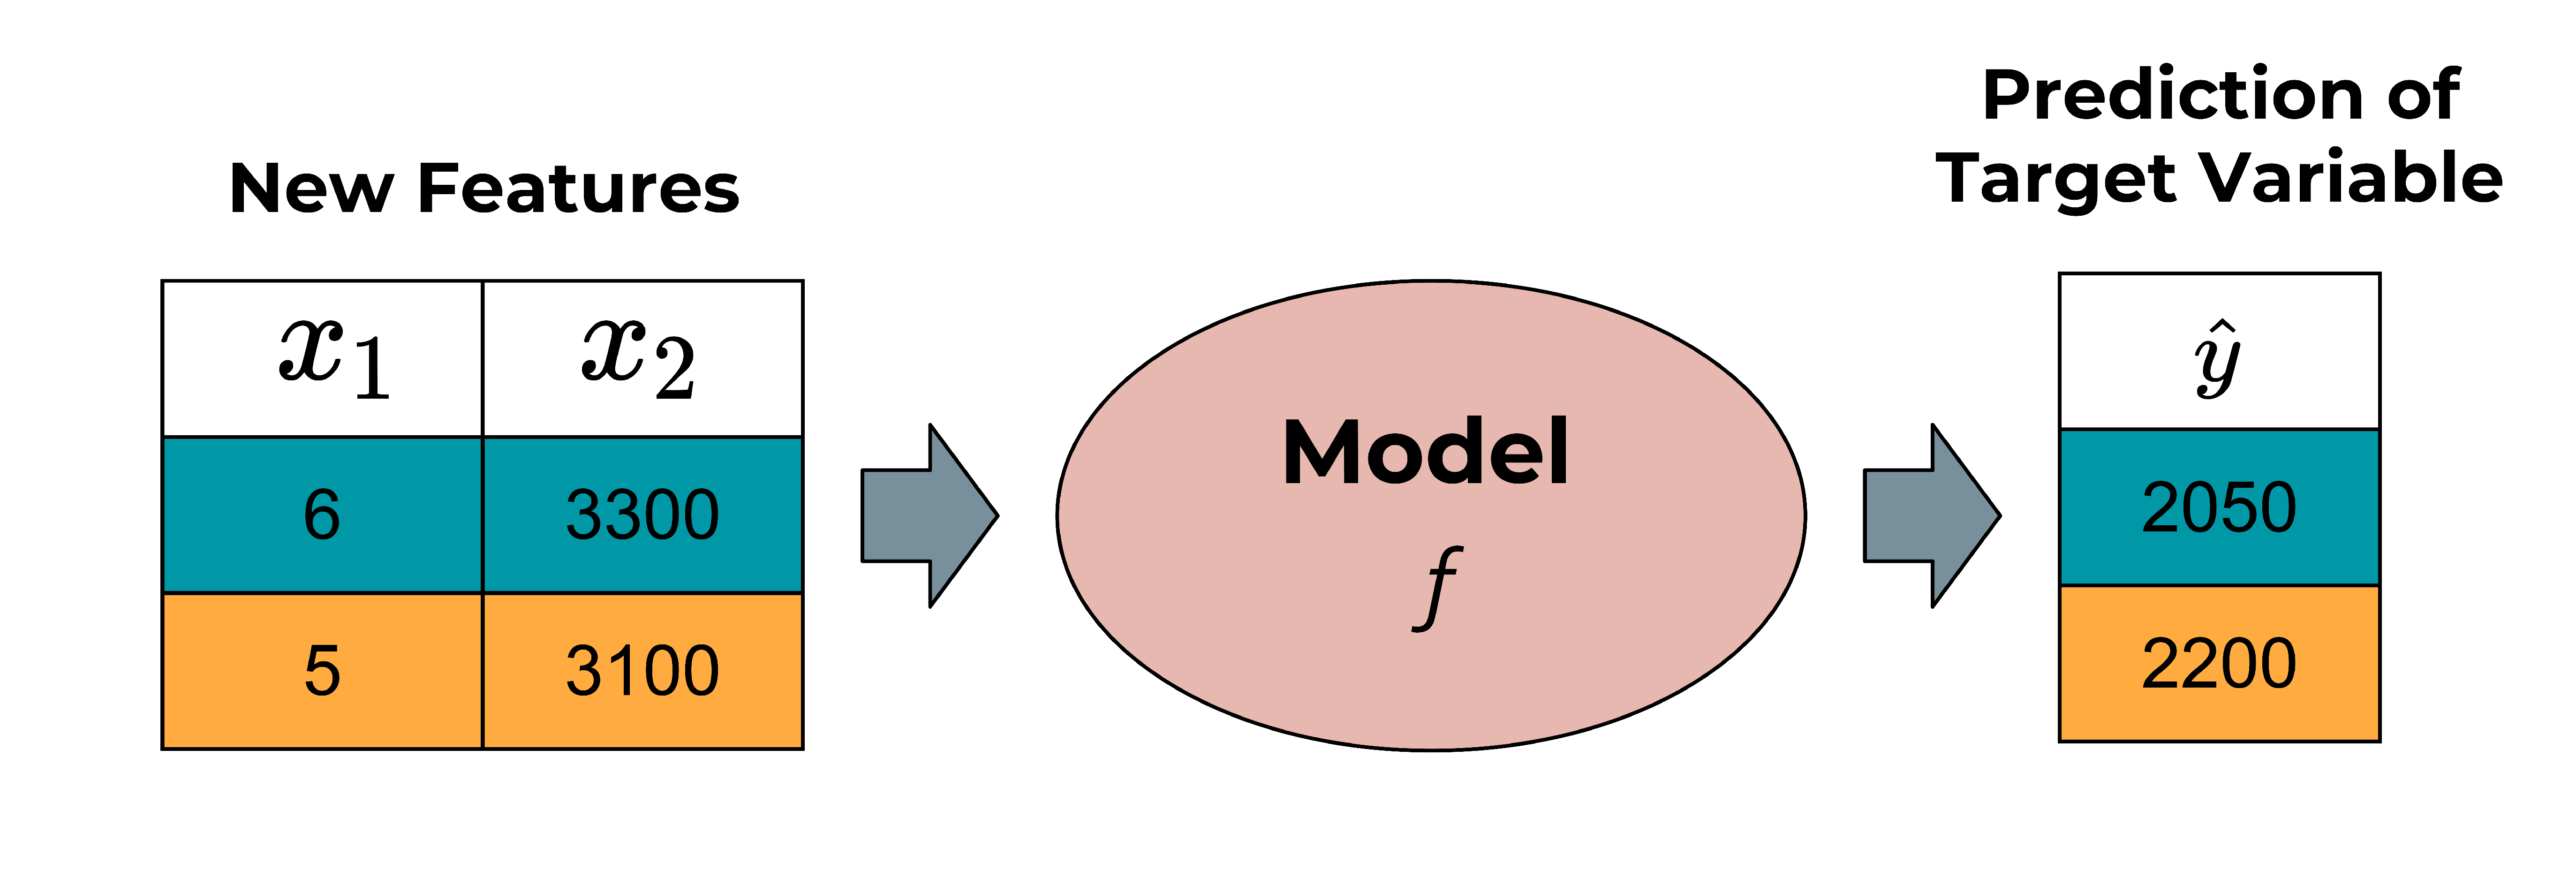
\includegraphics[width = 0.8\textwidth]{figure_man/the_model_web} 
\end{center}
  

\framebreak

\begin{itemize}

  \item $f$ is meant to capture intrinsic patterns of the data, the
  underlying assumption being that these hold true for \emph{all} data drawn 
  from $\Pxy$.
  
  \item It is easily conceivable how models can range from super simple (e.g., 
   linear, tree stumps) to very complex (e.g., deep neural networks) and there
   are infinitely many choices how we can construct such functions.
  
  \begin{figure}
  % \centering
  \begin{minipage}{0.4\textwidth}
    \centering
    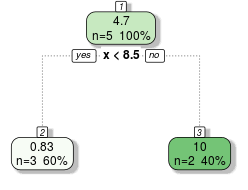
\includegraphics[width=0.8\linewidth]{figure_man/monotone_trafo1.png}
  \end{minipage}%
  \begin{minipage}{0.6\textwidth}
    \centering
    % Produced with Google Presentation
    % https://docs.google.com/presentation/d/13X6v1M7u3xkMUDCNNgtiFje2nAz8v5bW_bQhrQrx5To/edit#slide=id.p
    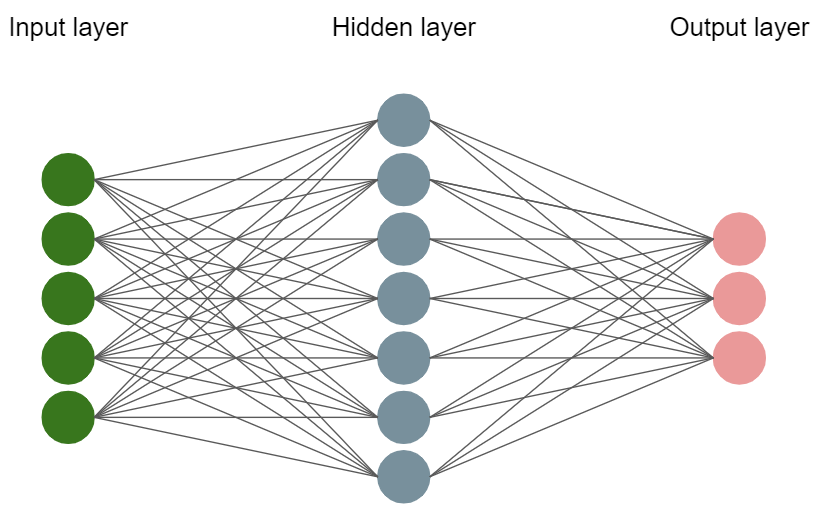
\includegraphics[width=0.8\linewidth]{figure_man/network.PNG}
  \end{minipage}
  \end{figure}
  
  \vspace{0.2cm}
  
  \item In fact, ML requires \textbf{constraining} $f$ to a   certain type of functions.

\end{itemize}

\end{vbframe}

% ------------------------------------------------------------------------------

\begin{vbframe}{Hypothesis Spaces}

\begin{itemize}

  \item Without restrictions on the functional family, the task of finding a 
  \enquote{good} model among all the available ones is impossible to solve.
  
  \item This means: we have to determine the class of our model \emph{a priori}, 
  thereby narrowing down our options considerably. We could call that a 
  \textbf{structural prior}.
  
  \item The set of functions defining a specific model class is called a 
  \textbf{hypothesis space} $\Hspace$:
  
  $$\Hspace = \{f: f \text{ belongs to a certain functional family}\}$$
  

\end{itemize}  

\end{vbframe}

% ------------------------------------------------------------------------------

\begin{vbframe}{Parametrization}

\begin{itemize}
  
  \item All models within one hypothesis space share a common functional 
  structure. We usually construct the space as 
  \textbf{parametrized family of curves}.
  
  % \item In fact, the only aspect in which they differ is the values of 
  % \textbf{parameters}.
  
  \item We collect all parameters in a \textbf{parameter vector} 
  $\thetab = (\theta_1, \theta_2, \ldots, \theta_d)$ from \textbf{parameter space} 
  $\Theta$.
  
  \item They are our means of fixing a specific function from the family. 
      Once set, our model is fully determined.
  
  \item Therefore, we can re-write $\Hspace$ as:

  \begin{equation*}
    \begin{split}
      \Hspace = \{f_{\thetab}: \quad & f_{\thetab} \text{ belongs to a certain
       functional family } \\
       & \text{parameterized by } \thetab\}
    \end{split}
  \end{equation*}
  
  
  \framebreak
  
  \item This means: finding the optimal model is perfectly equivalent to 
  finding the optimal set of parameter values.
  
  \item The relation between optimization over $f \in \Hspace$ and 
  optimization over $\thetab \in \Theta$ allows us to operationalize our search
  for the best model via the search for the optimal value on a $d$-dimensional
  parameter surface.
  
  \begin{center}
  % https://docs.google.com/presentation/d/1WoFzKsfmvVdkHJO0aEIN6U-DW-mglanIcPoW3d_Ecu0/edit#slide=id.p
    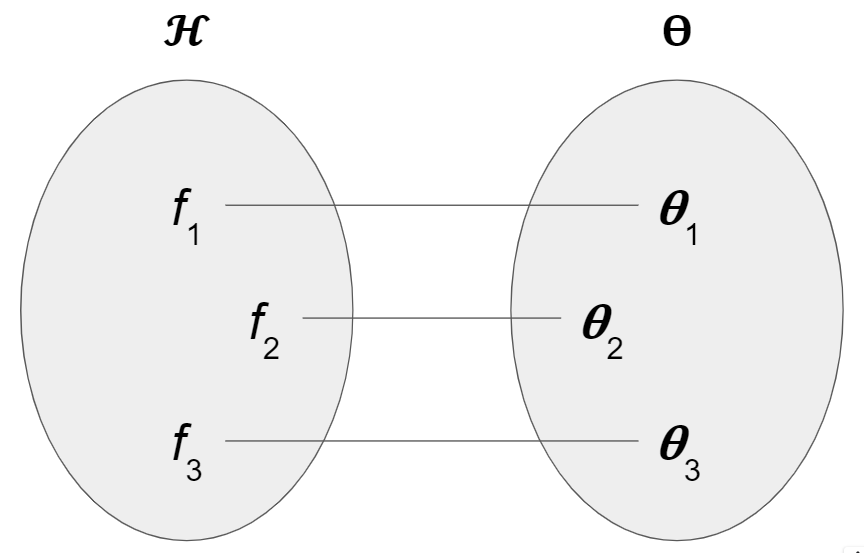
\includegraphics[width = 0.4\textwidth]{figure_man/bijection_f_theta.PNG} 
  \end{center}
  
  \item $\thetab$ might be scalar or comprise thousands of parameters,
  depending on the complexity of our model.
  

 \framebreak
  
  \item Short remark: In fact, some parameter vectors, for some model classes, might
      encode the same function. So the parameter-to-model mapping could 
      be non-injective. 
    \item We call this then a non-identifiable model.
    \item But this shall not concern us here.

  \begin{center}
% https://docs.google.com/presentation/d/1KYNhUr5SLH8mmLcgARAE4VRPFwYRytclpaSTLuKMuW0/edit#slide=id.p    
      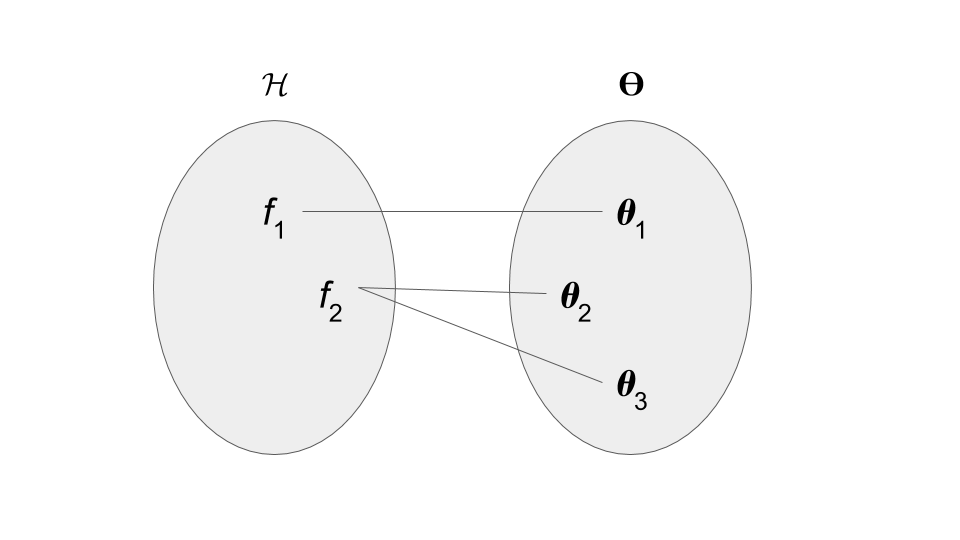
\includegraphics[width = 0.6\textwidth]{figure_man/bijection_f_theta_2.PNG} 
  \end{center}

\end{itemize}
\end{vbframe}

% ------------------------------------------------------------------------------

% \begin{vbframe}{Examples for Hypothesis Spaces}

\begin{vbframe}{Example: Univariate linear functions}
$$\Hspace = \{f: \fx = \textcolor{orange}{\theta_0} + 
\textcolor{blue}{\theta_1} x, \thetab \in \R^2\}$$

\begin{center}
  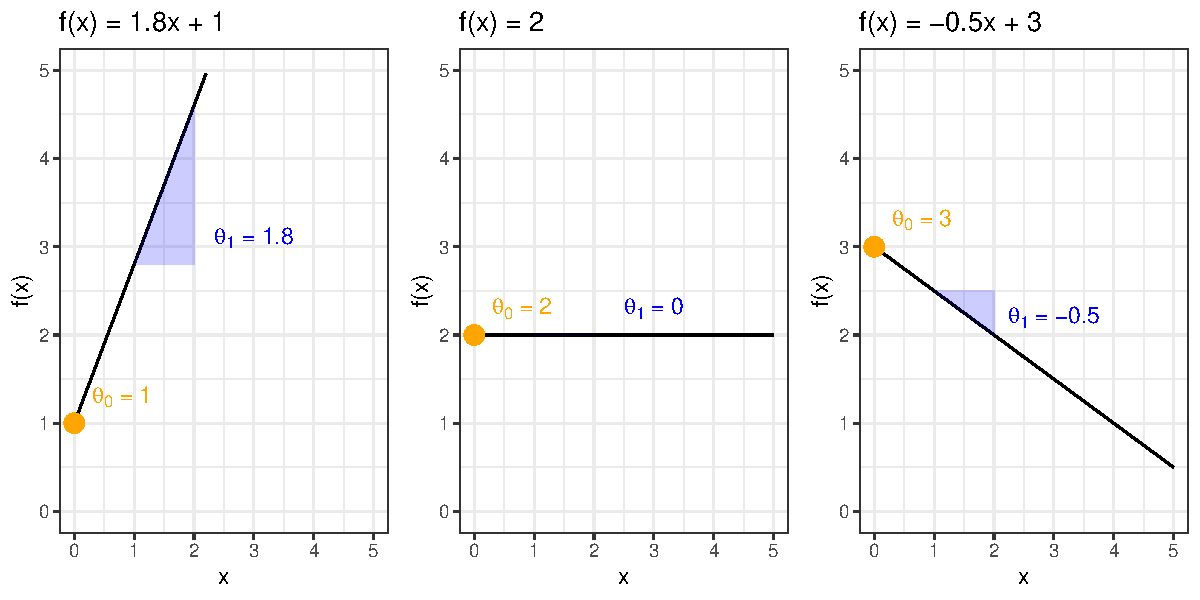
\includegraphics[width = \textwidth]{figure/hs-lin-functions.pdf}
\end{center}

\end{vbframe}

\begin{vbframe}{Example: Bivariate quadratic functions}

\begin{equation*}
  % \begin{split}
    \Hspace = \{f: \fx =  
        % \txtcolor{orange}{\theta_0} + \textcolor{blue}{p^T} 
    % \xv + \xv \textcolor{red}{Q} \xv^T =  \\
    \textcolor{orange}{\theta_0} + \textcolor{blue}{\theta_1} x_1 + 
    \textcolor{blue}{\theta_2} x_2 + \textcolor{red}{\theta_3} x_1^2 + 
    \textcolor{red}{\theta_4} x_2^2 + \textcolor{red}{\theta_5} x_1 x_2, 
    \thetab \in \R^6\},
  % \end{split}
\end{equation*}

% where 
% $p = \big(\begin{smallmatrix}
% \theta_1 & \theta_2
% \end{smallmatrix}\big)$
% and
% $Q = \Big(\begin{smallmatrix}
% \theta_3 & \frac{1}{2} \theta_5 \\
% \frac{1}{2} \theta_5 & \theta_4
% \end{smallmatrix}\Big).$

\vspace*{-\baselineskip}

\begin{columns}

  \tiny

  \begin{column}{0.33\textwidth}
    \begin{center}
      \begin{equation*}
        \begin{split}
          f(x) &= \textcolor{orange}{3} + \textcolor{blue}{2} x_1 + 
          \textcolor{blue}{4} x_2 \\
          \textcolor{white}{x} 
        \end{split}
      \end{equation*}
      \vspace*{-1.5\baselineskip}
      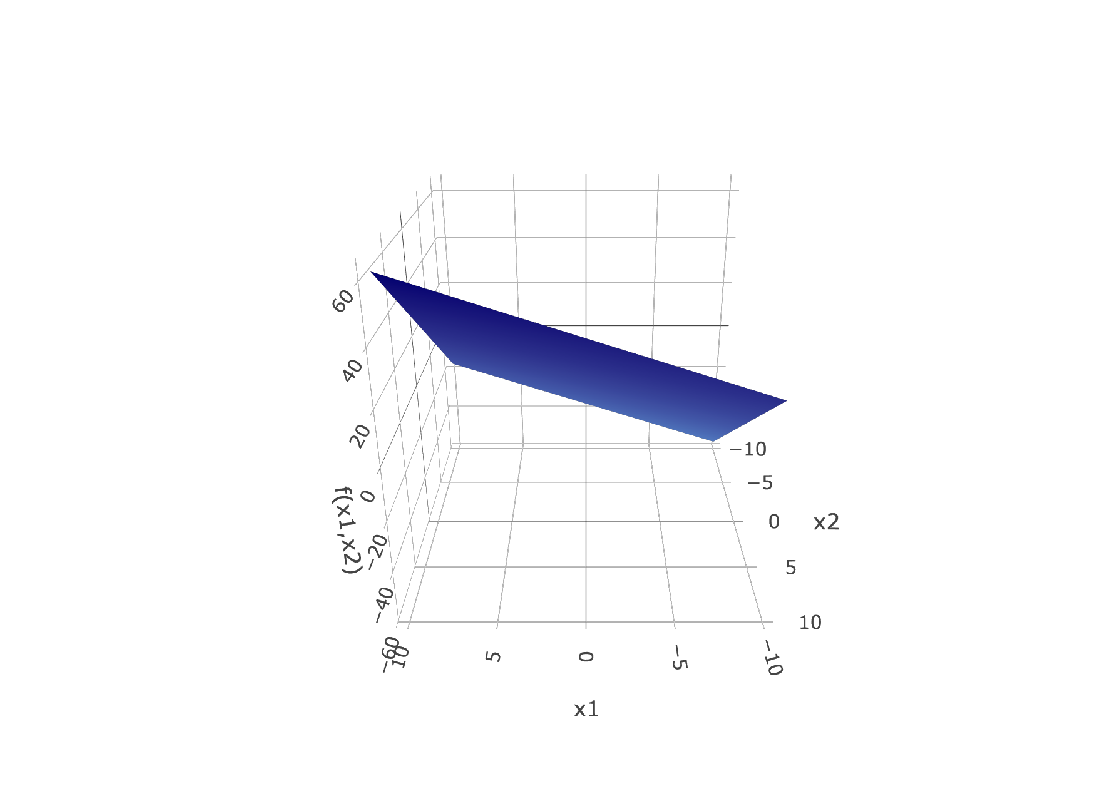
\includegraphics[trim = 100 10 100 50, clip, 
      width = \textwidth]{figure/hs-quadric-1.pdf}
    \end{center}
  \end{column}
  
  \begin{column}{0.33\textwidth}
    \begin{center}
      \begin{equation*}
        \begin{split}
          f(x) &= \textcolor{orange}{3} + \textcolor{blue}{2} x_1 + 
          \textcolor{blue}{4} x_2 + \\
          &+ \textcolor{red}{1} x_1^2 + \textcolor{red}{1} x_2^2
        \end{split}
      \end{equation*}
      \vspace*{-1.5\baselineskip}
      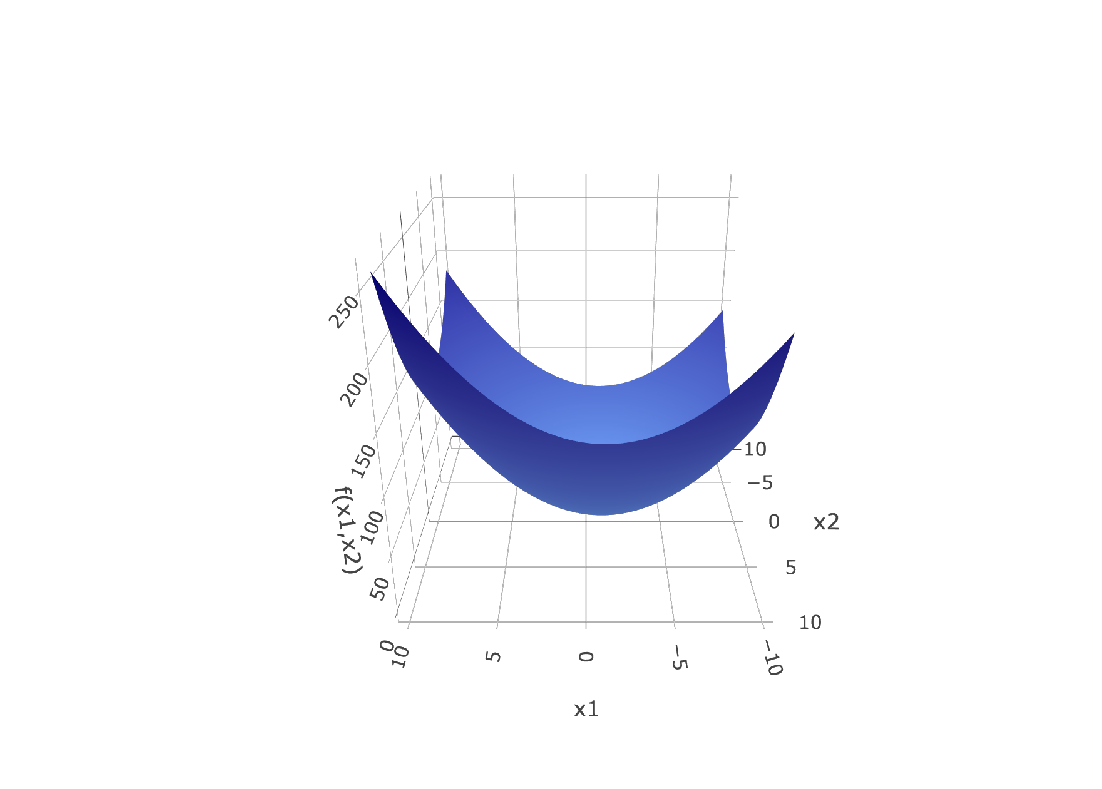
\includegraphics[trim = 100 10 100 50, clip, 
      width = \textwidth]{figure/hs-quadric-2.pdf}
    \end{center}
  \end{column}
  
  \begin{column}{0.33\textwidth}
    \begin{center}
      \begin{equation*}
        \begin{split}
          f(x) &= \textcolor{orange}{3} + \textcolor{blue}{2} x_1 + 
          \textcolor{blue}{4} x_2 + \\
          &+ \textcolor{red}{1} x_1^2 + \textcolor{red}{1} x_2^2 
          + \textcolor{red}{4} x_1 x_2
        \end{split}
      \end{equation*}
      \vspace*{-1.5\baselineskip}
      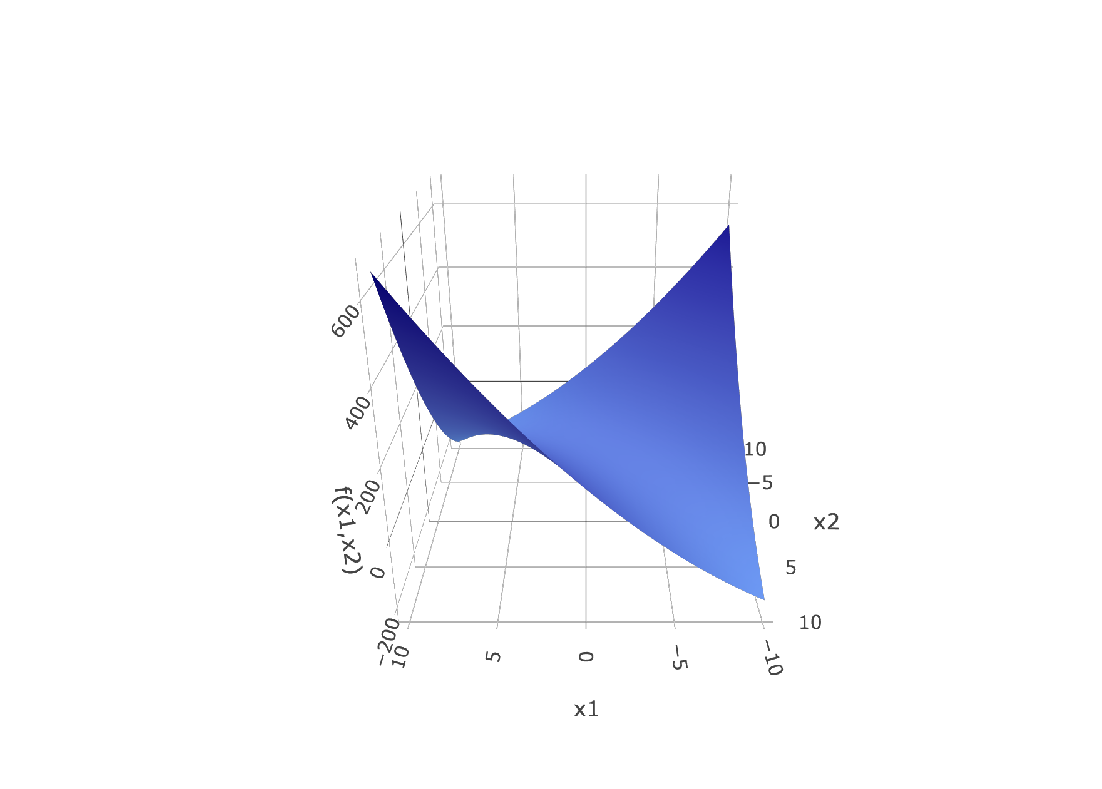
\includegraphics[trim = 100 10 100 50, clip, 
      width = \textwidth]{figure/hs-quadric-3.pdf}
    \end{center}
  \end{column}

  \normalsize
  
\end{columns}
\end{vbframe}


\begin{vbframe}{Example: RBF Network}
Radial basis function networks with Gaussian basis functions
$$\Hspace = \bigg\{ f: \fx =  \sumik \textcolor{blue}{a_i} \rho ( \| \xv - 
\textcolor{orange}{\textbf{c}_i}  \|) 
\bigg\},$$ 

\begin{minipage}{0.55\textwidth}
  \small
  where 
  \begin{itemize}
    \item $\textcolor{blue}{a_i}$ is the weight of the $i$-th neuron, 
    \item $\textcolor{orange}{\textbf{c}_i}$ its center vector, and
    \item $\rho( \| \xv - \textcolor{orange}{\textbf{c}_i} \|) = \exp(- \beta \| 
    \xv - \textcolor{orange}{\textbf{c}_i} \|^2)$ is the $i$-th radial basis
    function with bandwidth $\beta \in \R$.
  \end{itemize}
  Usually, the number of centers $k$ and the bandwidth $\beta$ need to be set 
  in advance (so-called \emph{hyperparameters}).
  \normalsize
\end{minipage}%
\begin{minipage}{0.45\textwidth}
    \centering
    % https://www.researchgate.net/figure/Structure-of-Stacked-Autoencoders_fig2_325025951
    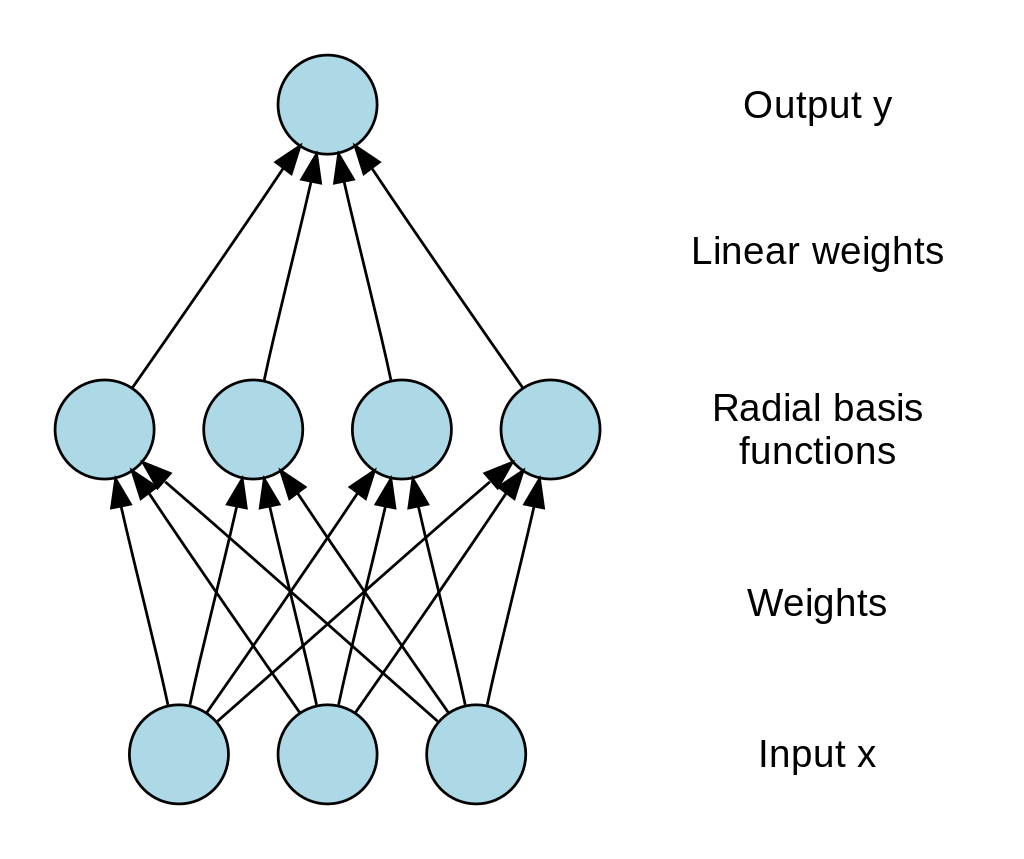
\includegraphics[width = 0.9\linewidth]{figure_man/rbf_network.png}
\end{minipage}

\framebreak

\begin{center}
  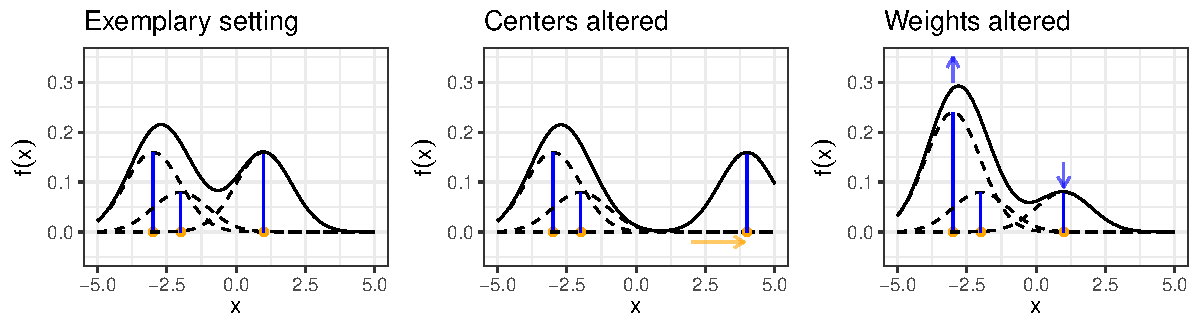
\includegraphics[width = \textwidth]{figure/hs-rbf-network-2d.pdf}
\end{center}

\tiny

\begin{minipage}{0.33\textwidth}
  \begin{center}
    $a_1 = 0.4, a_2 = 0.2, a_3 = 0.4$
    $c_1 = -3, c_2 = -2, c_3 = 1$
    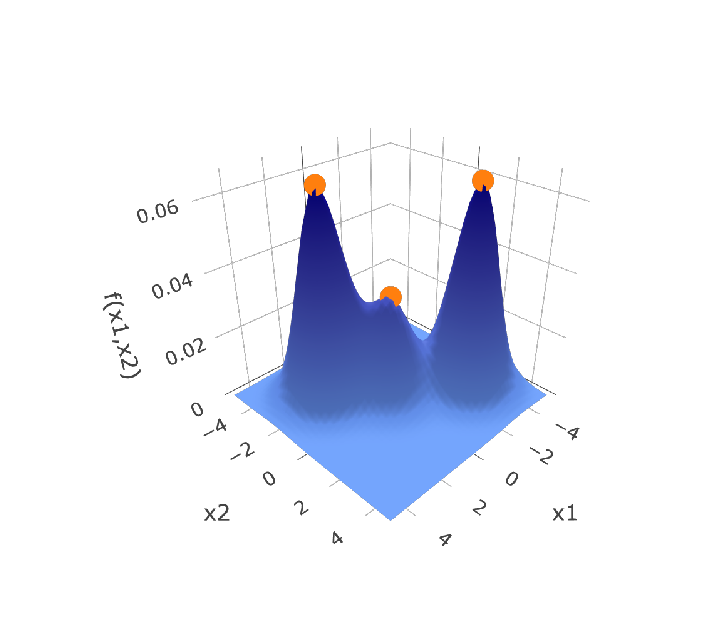
\includegraphics[trim = 50 30 50 50, clip, 
    width = \textwidth]{figure/hs-rbf-network-3d-1.pdf}
    $a_1 = 0.4, a_2 = 0.2, a_3 = 0.4$ \\
    $c_1 = (2,-2), c_2 = (0,0)$, \\
    $c_3 = (-3,2)$
  \end{center}
\end{minipage}%
\begin{minipage}{0.33\textwidth}
  \begin{center}
    $a_1 = 0.4, a_2 = 0.2, a_3 = 0.4$
    $c_1 = -3, c_2 = -2, \textcolor{orange}{c_3 = 1}$
    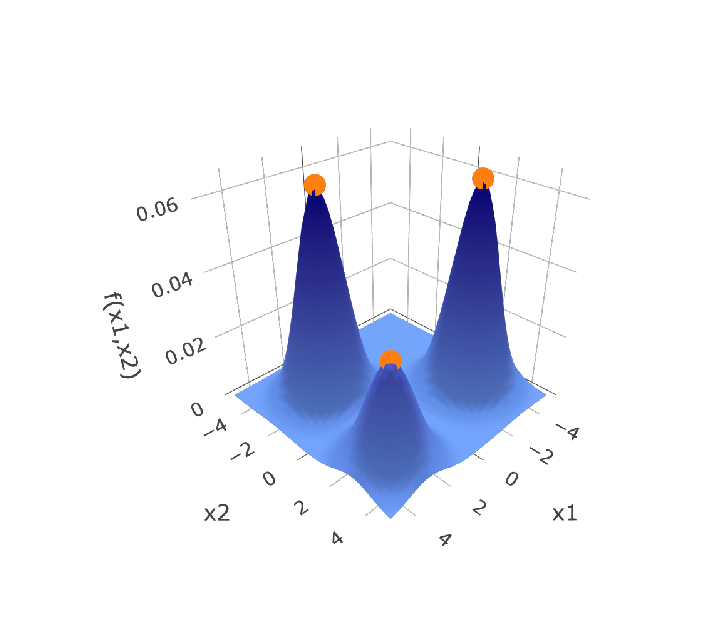
\includegraphics[trim = 50 30 50 50, clip, 
    width = \textwidth]{figure/hs-rbf-network-3d-2.pdf}
    $a_1 = 0.4, a_2 = 0.2, a_3 = 0.4$ \\
    $c_1 = (2,-2), \textcolor{orange}{c_2 = (3,3)},$ \\
    $c_3 = (-3,2)$
  \end{center}
\end{minipage}%
\begin{minipage}{0.33\textwidth}
  \begin{center}
    $\textcolor{blue}{a_1 = 0.6}, a_2 = 0.2, \textcolor{blue}{a_3 = 0.2}$
    $c_1 = -3, c_2 = -2, c_3 = 1$
    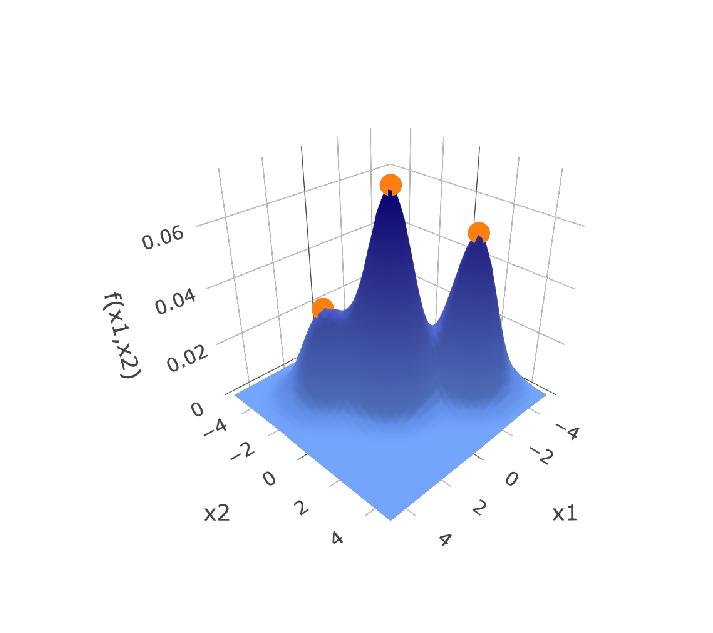
\includegraphics[trim = 50 30 50 50, clip, 
    width = \textwidth]{figure/hs-rbf-network-3d-3.pdf}
    $\textcolor{blue}{a_1 = 0.2, a_2 = 0.45, a_3 = 0.35}$
    $c_1 = (2,-2), c_2 = (0,0),$ \\
    $c_3 = (-3,2)$
  \end{center}
\end{minipage}

\normalsize

% \framebreak
% 
% 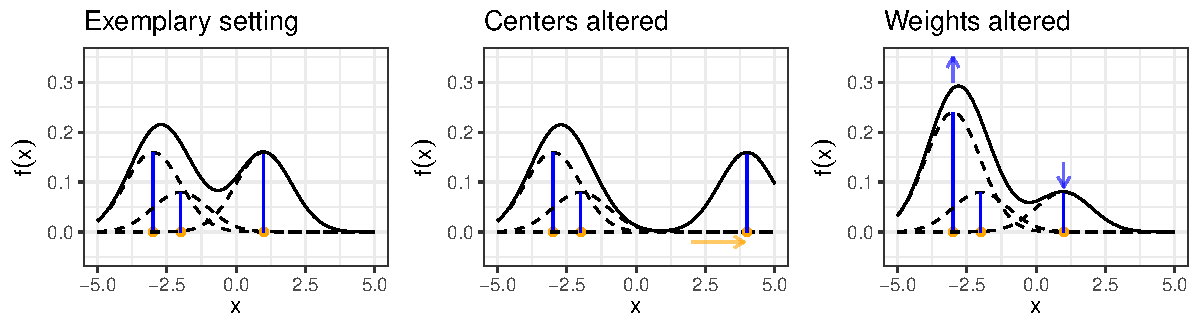
\includegraphics[width = \textwidth]{figure/hs-rbf-network-2d.pdf}
% 
% \footnotesize
% 
% \begin{minipage}{0.33\textwidth}
%   \begin{center}
%     \begin{equation*}
%       \begin{split}
%         a_1 &= 0.4 \\
%         a_2 &= 0.2 \\
%         a_3 &= 0.4 \\
%         c_1 &= -3 \\
%         c_2 &= -2 \\
%         c_3 &= 1
%       \end{split}
%     \end{equation*}
%   \end{center}
% \end{minipage}%
% \begin{minipage}{0.33\textwidth}
%   \begin{center}
%     \begin{equation*}
%       \begin{split}
%         a_1 &= 0.4 \\
%         a_2 &= 0.2 \\
%         a_3 &= 0.4 \\
%         c_1 &= -3 \\
%         c_2 &= -2 \\
%         \textcolor{orange}{c_3} & \textcolor{orange}{=} \textcolor{orange}{1}
%       \end{split}
%     \end{equation*}
%   \end{center}
% \end{minipage}%
% \begin{minipage}{0.33\textwidth}
%   \begin{center}
%     \begin{equation*}
%       \begin{split}
%         \textcolor{blue}{a_1} & \textcolor{blue}{=} \textcolor{blue}{0.6} \\
%         a_2 &= 0.2 \\
%         \textcolor{blue}{a_3} & \textcolor{blue}{=} \textcolor{blue}{0.2} \\
%         c_1 &= -3 \\
%         c_2 &= -2 \\
%         c_3 &= 1
%       \end{split}
%     \end{equation*}
%   \end{center}
% \end{minipage}
% 
% \normalsize
% 
% \framebreak
% 
% % \vspace*{-\baselineskip}
% 
% \footnotesize
% 
% \begin{minipage}{0.33\textwidth}
%   \begin{center}
%       Exemplary setting
%       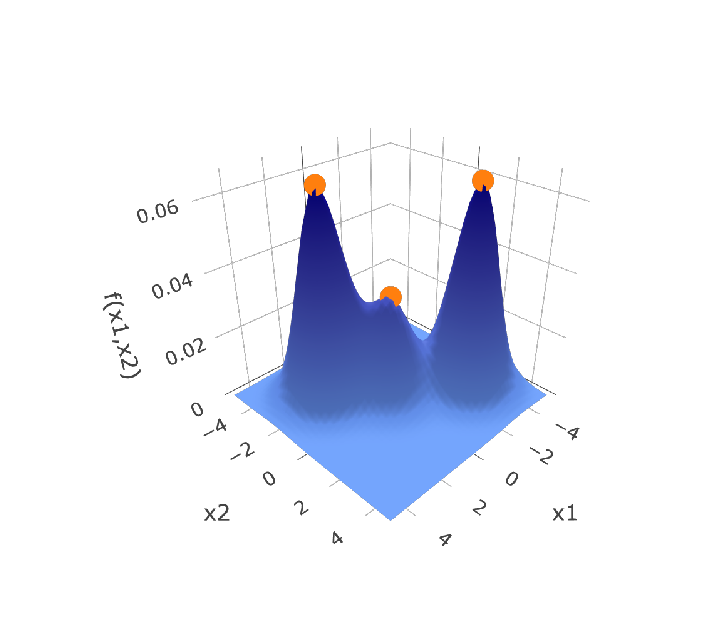
\includegraphics[width=\textwidth]{figure/hs-rbf-network-3d-1.pdf}
%       \begin{equation*}
%         \begin{split}
%           a_1 &= 0.4 \\
%           a_2 &= 0.2 \\
%           a_3 &= 0.4 \\
%           c_1 &= (2,-2) \\
%           c_2 &= (0,0) \\
%           c_3 &= (-3,2)
%         \end{split}
%       \end{equation*}
%     \end{center}
% \end{minipage}%
% \begin{minipage}{0.33\textwidth}
%   \begin{center}
%       Centers altered
%       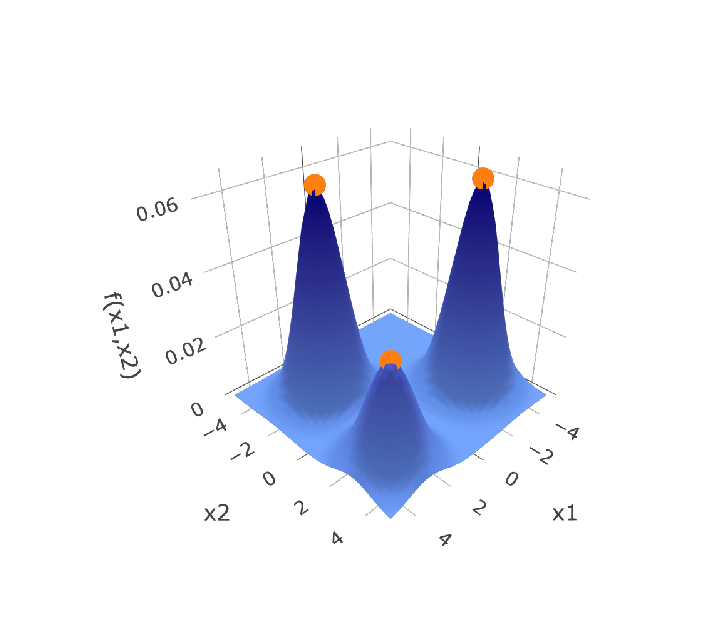
\includegraphics[width=1\textwidth]{figure/hs-rbf-network-3d-2.pdf}
%       \begin{equation*}
%         \begin{split}
%           a_1 &= 0.4 \\
%           a_2 &= 0.2 \\
%           a_3 &= 0.4 \\
%           c_1 &= (2,-2) \\
%           \textcolor{orange}{c_2} & \textcolor{orange}{=}
%           \textcolor{orange}{(3,3)} \\
%           c_3 &= (-3,2)
%         \end{split}
%       \end{equation*}
%     \end{center}
% \end{minipage}%
% \begin{minipage}{0.33\textwidth}
%   \begin{center}
%       Weights altered
%       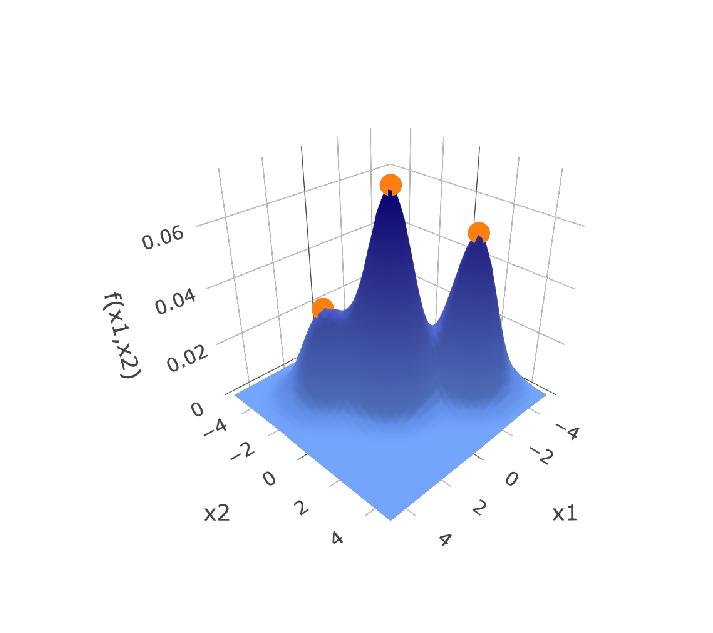
\includegraphics[width=1\textwidth]{figure/hs-rbf-network-3d-3.pdf}
%       \begin{equation*}
%         \begin{split}
%           \textcolor{blue}{a_1} & \textcolor{blue}{=} \textcolor{blue}{0.2} \\
%           \textcolor{blue}{a_2} & \textcolor{blue}{=} \textcolor{blue}{0.45} \\
%           \textcolor{blue}{a_3} & \textcolor{blue}{=} \textcolor{blue}{0.35} \\
%           c_1 &= (2,-2) \\
%           c_2 &= (0,0) \\
%           c_3 &= (-3,2)
%         \end{split}
%       \end{equation*}
%     \end{center}
% \end{minipage}
% 
% \normalsize

\end{vbframe}

% ------------------------------------------------------------------------------

\endlecture
\end{document}
